\documentclass[10pt,a4paper]{article}

% ==============================================================================
% Packages & Configuration
% ==============================================================================
\usepackage[utf8]{inputenc}
\usepackage[T1]{fontenc}
\usepackage{lmodern}
\usepackage[margin=1.75cm,top=1.75cm,bottom=1.75cm]{geometry}
\usepackage{amsmath,amssymb,amsfonts}
\usepackage{graphicx}
\usepackage{xcolor}
\usepackage{booktabs}
\usepackage{tabularx}
\usepackage{array}
\usepackage{enumitem}
\usepackage{microtype}
\usepackage{titlesec}
\usepackage{fancyhdr}
\usepackage{lastpage}
\usepackage{caption}
\usepackage{tikz}
\usetikzlibrary{shapes.geometric, arrows.meta, positioning, calc, fit, backgrounds}
\usepackage[most]{tcolorbox}
\usepackage{hyperref}

% Display math spacing
\setlength{\abovedisplayskip}{3pt plus 1pt minus 1pt}
\setlength{\belowdisplayskip}{3pt plus 1pt minus 1pt}

% Color Palette (Academic / Engineering)
\definecolor{primaryblue}{RGB}{27, 54, 93}       % Deep Navy
\definecolor{secondaryblue}{RGB}{41, 128, 185}   % Cobalt Blue
\definecolor{accentorange}{RGB}{211, 84, 0}      % Hazard Amber
\definecolor{darkslate}{RGB}{44, 62, 80}         % Charcoal
\definecolor{lightgraybg}{RGB}{248, 249, 250}    % Soft Canvas Gray
\definecolor{bordergray}{RGB}{220, 224, 230}     % Border Gray
\definecolor{forestgreen}{RGB}{39, 110, 68}      % Eco Green
\definecolor{hazardred}{RGB}{180, 40, 30}        % Hazard Red

% Hyperref Setup
\hypersetup{
    colorlinks=true,
    linkcolor=primaryblue,
    citecolor=secondaryblue,
    urlcolor=secondaryblue,
    pdftitle={Autonomous Bimanual Hazardous E-Waste Triage: Disposable Vape Detection and Extraction},
    pdfauthor={Leukerbad Hackathon 2026 Robotics Team}
}

% Section Titles Styling
\titleformat{\section}
  {\color{primaryblue}\large\bfseries}
  {\thesection.}{0.4em}{}[\titlerule]
\titleformat{\subsection}
  {\color{darkslate}\normalsize\bfseries}
  {\thesubsection}{0.4em}{}
\titleformat{\subsubsection}
  {\color{secondaryblue}\small\bfseries}
  {\thesubsubsection}{0.4em}{}

\titlespacing*{\section}{0pt}{0.65ex plus .2ex minus .1ex}{0.25ex plus .1ex}
\titlespacing*{\subsection}{0pt}{0.5ex plus .2ex minus .1ex}{0.2ex plus .1ex}
\titlespacing*{\subsubsection}{0pt}{0.35ex plus .1ex minus .1ex}{0.15ex plus .1ex}

% Caption Styling
\captionsetup{font=small,labelfont={bf,color=primaryblue},skip=2.5pt}

% Header & Footer
\pagestyle{fancy}
\fancyhf{}
\renewcommand{\headrulewidth}{0.4pt}
\renewcommand{\footrulewidth}{0.4pt}
\fancyhead[L]{\footnotesize\color{darkslate}\textbf{Leukerbad Robotics Hackathon 2026} \textbar\ Robotics, XR \& AI Track}
\fancyhead[R]{\footnotesize\color{darkslate}Autonomous Bimanual Hazardous E-Waste Triage}
\fancyfoot[L]{\footnotesize\color{darkslate}Technical Overview \& System Specification}
\fancyfoot[R]{\footnotesize\color{darkslate}Page \thepage\ of \pageref{LastPage}}

% Custom Callout Box
\newtcolorbox{calloutbox}[2][]{
    colback=lightgraybg,
    colframe=primaryblue,
    fonttitle=\bfseries\color{white},
    coltitle=white,
    title=#2,
    arc=1.5mm,
    boxrule=0.7pt,
    left=2.5mm, right=2.5mm, top=1.2mm, bottom=1.2mm,
    #1
}

% Compact list settings
\setlist{itemsep=0.4pt, topsep=0.8pt, parsep=0pt, leftmargin=1.2em}

% ==============================================================================
% Document Start
% ==============================================================================
\begin{document}

% ==============================================================================
% PAGE 1: Title, Abstract, Motivation, & Bimanual Strategy Introduction
% ==============================================================================

\begin{center}
    {\Large\bfseries\color{primaryblue} Autonomous Bimanual Hazardous E-Waste Triage:}\\[0.18em]
    {\large\bfseries\color{secondaryblue} Disposable Vape Detection \& Extraction with Dual SO-101 Manipulators}\\[0.25em]
    {\small\textbf{Leukerbad Hackathon 2026: Robotics, XR \& AI Track}}\\[0.12em]
    {\footnotesize\color{darkslate} Engineering Technical Report \textbar\ Dual SO-101 Open-Source Manipulator Platform \textbar\ Apple Silicon / ROS 2 / PyTorch}
\end{center}
\vspace{-0.65em}
\hrule height 1.0pt
\vspace{0.45em}

\begin{abstract}
\noindent
Disposable electronic cigarettes (``puffs'') represent one of the fastest-growing and most ecologically damaging municipal hazardous waste crises in Europe, discarding millions of intact, combustible lithium-ion pouch cells into standard recycling and municipal solid waste streams weekly. When compacted in garbage trucks or sorting trommels, these batteries suffer mechanical puncture, igniting severe thermal runaway fires and leaching heavy metals and nicotine. We introduce an autonomous, open-source robotic triage cell deploying dual 6-DOF SO-101 manipulators for coordinated clearing and hazardous extraction. The perception system implements a two-stage \textbf{System 1 / System 2} architecture: System 1 leverages a real-time \textbf{YOLOv11-seg} instance segmentation model (${\sim}15\,\text{ms}$ on Apple Silicon MPS) paired with an analytical \textbf{Rotating Calipers} minimum-area oriented bounding box (OBB) grasp planner, bypassing neural angle wrap-around ambiguities; System 2 integrates a toggleable \textbf{Gemini 2.5 Flash} Multimodal Large Language Model (VLM) verifier operating over unconstrained native-resolution crops to overcome closed-set shortcut learning and reject adversarial lookalikes (AirPods, highlighters, lighters). Tested across a comprehensive two-stage transfer dataset with zero-shot device generalization and logged physical grasp verification, this system establishes a low-cost, production-viable solution for municipal hazardous e-waste isolation.
\end{abstract}
\vspace{-0.3em}

\section{Motivation \& Hackathon Track Alignment}

\subsection{The Municipal Hazardous Waste Crisis: Disposable Vapes (``Puffs'')}
In recent years, the consumption of single-use disposable vapes has escalated exponentially. Each disposable unit consists of a high-energy-density $3.7\,\text{V}$ lithium-ion battery ($350$--$650\,\text{mAh}$), synthetic nicotine salt e-liquid reservoir, resistive heating coil, micro-sensor, and polymer/aluminum shell. Despite being manufactured as throwaway items, they represent fully functional electronics containing critical raw materials (lithium, cobalt, nickel, and copper).
\begin{itemize}
    \item \textbf{Thermal Runaway Deflagrations:} When mixed with municipal solid waste (MSW) or household recyclables, disposable vapes undergo mechanical crushing in compaction trucks, shredders, and ballistic separators. Internal short-circuits trigger violent thermal runaway ($T > 600^\circ\text{C}$), causing catastrophic fires in municipal recycling facilities and collection fleets.
    \item \textbf{Ecotoxicological Leaching:} Residual e-liquids contain concentrated nicotine salts, propylene glycol, and dissolved heavy metals (lead, cadmium, chromium), threatening groundwater contamination and soil degradation when landfilled.
    \item \textbf{Critical Mineral Dissipation:} Millions of tons of virgin battery-grade lithium and refined cobalt are permanently lost from circular supply chains due to lack of specialized singulation and disassembly infrastructure.
\end{itemize}

\subsection{Direct Alignment with Leukerbad Hackathon 2026 Tracks}
The project directly addresses three core challenges delineated by the Leukerbad Robotics Hackathon:
\begin{enumerate}
    \item \textbf{Sustainable Urban Development:} Facilitates urban circular economy loops by recovering high-purity lithium cells before contamination, supporting Switzerland's strict e-waste recovery guidelines (VREG/ORDEE).
    \item \textbf{Resilient \& Safe Cities:} Mitigates structural fire risks at municipal sorting infrastructure through early-stage, automated removal of volatile electrochemical hazards from open waste conveyors.
    \item \textbf{Autonomous Urban Services:} Demonstrates decentralizable, low-cost autonomous robotic infrastructure operating locally on edge compute (Apple Silicon Metal Performance Shaders) without reliance on heavy industrial PLCs.
\end{enumerate}

\section{Bimanual Hardware Strategy: Dual SO-101 Manipulators}

Industrial waste sorting requires handling extreme clutter, occlusion, and varied physical form factors. A single manipulator rapidly suffers from spatial bottlenecks when attempting to both clear non-hazardous debris and execute delicate antipodal grasps. We deploy a coordinated bimanual workstation utilizing two 6-DOF \textbf{SO-101} open-source robotic arms mounted on opposite flanks of the triage table (Figure~\ref{fig:hardware_layout}).

\subsection{Bimanual Role Partition}
\begin{itemize}
    \item \textbf{Arm 1 (The Forager / Singulator):} Dedicated to coarse workspace management. It dynamically sweeps aside non-hazardous occluding objects (crumpled paper, cardboard sleeves, beverage cans) and performs singulation pushes on dense debris clusters to separate touching objects, exposing hidden vapes to the vision system.
    \item \textbf{Arm 2 (The Hazmat Extractor):} Dedicated exclusively to precision extraction. Equipped with high-friction silicone-padded parallel jaws, Arm 2 receives validated SE(2) grasp poses from the perception engine, aligns its wrist orientation with the target's minor antipodal axis, grasps the vape body, and transfers it to a fire-safe containment vessel buffered with vermiculite.
\end{itemize}

\newpage
% ==============================================================================
% PAGE 2: Hardware Diagram, Calibration, & System 1 Instance Segmentation
% ==============================================================================

\begin{center}
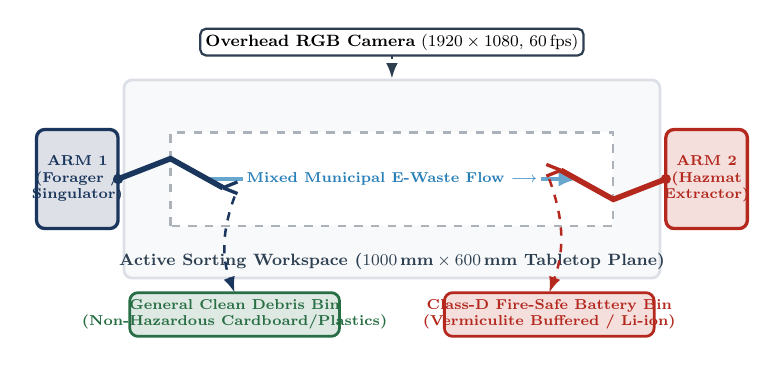
\begin{tikzpicture}[scale=0.74, every node/.style={transform shape}]
    % Table workspace
    \draw[fill=lightgraybg, draw=bordergray, line width=1pt, rounded corners=3pt] (-4.6,-1.7) rectangle (4.6,1.7);
    \node[text=darkslate, font=\bfseries\footnotesize] at (0, -1.42) {Active Sorting Workspace ($1000\,\text{mm} \times 600\,\text{mm}$ Tabletop Plane)};

    % Conveyor / Waste Flow
    \draw[fill=white, draw=darkslate!40, dashed, line width=0.8pt] (-3.8,-0.8) rectangle (3.8,0.8);
    \draw[-{Latex[length=2.5mm]}, line width=1.5pt, color=secondaryblue!70] (-3.2,0) -- (3.2,0);
    \node[fill=white, inner sep=2pt, font=\scriptsize\bfseries, text=secondaryblue] at (0,0) {Mixed Municipal E-Waste Flow $\longrightarrow$};

    % Arm 1: Forager / Singulator
    \draw[fill=primaryblue!15, draw=primaryblue, line width=1.2pt, rounded corners=3pt] (-6.1,-0.85) rectangle (-4.7,0.85);
    \node[align=center, font=\scriptsize\bfseries, text=primaryblue, inner sep=2pt] at (-5.4, 0) {ARM 1\\(Forager /\\Singulator)};
    \draw[fill=primaryblue, draw=none] (-4.7,0) circle (2.5pt);
    \draw[line width=2pt, color=primaryblue] (-4.7,0) -- (-3.8, 0.35) -- (-2.9, -0.15);
    \draw[line width=1.2pt, color=primaryblue] (-2.9,-0.15) -- (-2.65, -0.05);
    \draw[line width=1.2pt, color=primaryblue] (-2.9,-0.15) -- (-2.65, -0.25);

    % Arm 2: Hazmat Extractor
    \draw[fill=hazardred!15, draw=hazardred, line width=1.2pt, rounded corners=3pt] (4.7,-0.85) rectangle (6.1,0.85);
    \node[align=center, font=\scriptsize\bfseries, text=hazardred, inner sep=2pt] at (5.4, 0) {ARM 2\\(Hazmat\\Extractor)};
    \draw[fill=hazardred, draw=none] (4.7,0) circle (2.5pt);
    \draw[line width=2pt, color=hazardred] (4.7,0) -- (3.8, -0.35) -- (2.9, 0.15);
    \draw[line width=1.2pt, color=hazardred] (2.9,0.15) -- (2.65, 0.25);
    \draw[line width=1.2pt, color=hazardred] (2.9,0.15) -- (2.65, 0.05);

    % Overhead Camera
    \node[draw=darkslate, fill=white, line width=0.8pt, rounded corners=2pt, inner sep=2.5pt] (cam) at (0, 2.35) {\footnotesize\textbf{Overhead RGB Camera} ($1920\times1080$, $60\,\text{fps}$)};
    \draw[-{Latex[length=2mm]}, dotted, line width=1pt, color=darkslate] (cam.south) -- (0, 1.72);

    % Receptacles
    \draw[fill=forestgreen!15, draw=forestgreen, line width=1pt, rounded corners=3pt] (-4.5,-2.7) rectangle (-0.9,-1.95);
    \node[font=\scriptsize\bfseries, text=forestgreen, align=center, inner sep=2pt] at (-2.7,-2.32) {General Clean Debris Bin\\(Non-Hazardous Cardboard/Plastics)};

    \draw[fill=hazardred!15, draw=hazardred, line width=1pt, rounded corners=3pt] (0.9,-2.7) rectangle (4.5,-1.95);
    \node[font=\scriptsize\bfseries, text=hazardred, align=center, inner sep=2pt] at (2.7,-2.32) {Class-D Fire-Safe Battery Bin\\(Vermiculite Buffered / Li-ion)};

    % Action arrows
    \draw[-{Latex[length=2mm]}, dashed, color=primaryblue, line width=0.9pt] (-2.7,-0.3) to [bend right=20] (-2.7,-1.95);
    \draw[-{Latex[length=2mm]}, dashed, color=hazardred, line width=0.9pt] (2.7,0.0) to [bend left=20] (2.7,-1.95);
\end{tikzpicture}
\captionof{figure}{Dual SO-101 bimanual coordination layout illustrating the complementary task partition: Arm 1 clears occluding inert materials while Arm 2 executes high-precision antipodal extraction of combustible e-cigarettes into vermiculite-buffered containment.}
\label{fig:hardware_layout}
\end{center}
\vspace{-0.4em}

\subsection{Overhead Coordinate Calibration via Planar Homography}
A single calibrated overhead sensor (Logitech Brio / Intel RealSense D435) provides top-down orthographic visual coverage of the workspace. Because the triage surface is a fixed planar manifold $Z = Z_{\text{table}}$, image coordinates $(u, v)$ map to robot base coordinates $(X, Y)$ via a planar homography matrix $H \in \mathbb{R}^{3\times3}$:
\begin{equation}
    s \begin{bmatrix} X \\ Y \\ 1 \end{bmatrix} = H \begin{bmatrix} u \\ v \\ 1 \end{bmatrix}, \quad \text{where } H = \begin{bmatrix} h_{11} & h_{12} & h_{13} \\ h_{21} & h_{22} & h_{23} \\ h_{31} & h_{32} & 1 \end{bmatrix}
\end{equation}
The matrix $H$ is estimated offline using a $7\times9$ ChArUco fiducial calibration grid with sub-millimeter reprojection error ($\text{RMSE} < 0.42\,\text{mm}$). Full 6-DOF execution poses are constructed as:
\begin{equation}
    \mathbf{T}_{\text{grasp}} = \begin{bmatrix} 
    \cos\theta_{\text{grasp}} & -\sin\theta_{\text{grasp}} & 0 & X_{\text{target}} \\
    \sin\theta_{\text{grasp}} & \cos\theta_{\text{grasp}} & 0 & Y_{\text{target}} \\
    0 & 0 & -1 & Z_{\text{table}} + \delta_{\text{clearance}} \\
    0 & 0 & 0 & 1 
    \end{bmatrix}
\end{equation}

\section{Perception Architecture: Fast System 1 \& Verifying System 2}

\subsection{Why Axis-Aligned Bounding Boxes Fail on Cylindrical E-Waste}
Standard object detection frameworks (e.g., standard YOLO bounding boxes) predict axis-aligned rectangles $[x_{\min}, y_{\min}, x_{\max}, y_{\max}]$. For arbitrary-angle cylindrical vapes ($0^\circ \le \theta \le 180^\circ$), axis-aligned boxes suffer fatal geometric failure modes:
\begin{enumerate}
    \item \textbf{Excess Background Inclusion:} A $45^\circ$-rotated vape of length $120\,\text{mm}$ and width $20\,\text{mm}$ results in a bounding box that is ${\sim}85\,\text{mm} \times 85\,\text{mm}$. Over $70\%$ of the bounding area comprises irrelevant background or neighboring clutter.
    \item \textbf{Loss of Principal Orientation:} The axis-aligned box provides zero information regarding whether the object lies along the $+45^\circ$ or $-45^\circ$ diagonal, preventing antipodal gripper alignment.
    \item \textbf{Centroid Drift in Overlapping Scenarios:} Cluttered adjacent items within the box corrupt center-of-mass estimation, causing the parallel-jaw gripper to collide with adjacent debris or crush the fragile battery shell.
\end{enumerate}
Consequently, pixel-accurate instance segmentation ($M_i \subset \mathbb{R}^{H \times W}$) is strictly necessary for robotic grasp planning.

\subsection{System 1: Real-Time Instance Segmentation (\texttt{YOLOv11-seg})}
We deploy \texttt{yolo11s-seg}, fine-tuned specifically for single-use e-cigarettes. The model architecture features:
\begin{itemize}
    \item \textbf{Backbone \& Neck:} Modified CSPNet featuring cross-stage partial blocks with kernel sizes $k=2,3$ (\texttt{C3k2}), complemented by Path Aggregation Network (PANet) and a \texttt{C2PSA} (Convolutional Cross-Stage Partial with Spatial Attention) block to enhance feature saliency for slender, reflective metallic/plastic cylinders.
    \item \textbf{YOLACT-Style Dual Prototype Mask Branch:} Rather than predicting masks via heavy instance-specific decoders, the network outputs $k=32$ global mask prototype bases $P \in \mathbb{R}^{k \times \frac{H}{4} \times \frac{W}{4}}$ from the P3 feature map, and a vector of 32 mask coefficients $\mathbf{c}_i \in \mathbb{R}^{32}$ per detected bounding proposal. The final binary mask for instance $i$ is generated by linear combination and sigmoid activation:
    \begin{equation}
        M_i(x, y) = \sigma\left( \sum_{m=1}^{32} c_{i,m} \cdot P_m(x, y) \right) \ge \tau_{\text{mask}}, \quad \tau_{\text{mask}} = 0.5
    \end{equation}
    \item \textbf{Inference Performance:} On an Apple M-series Silicon processor utilizing Metal Performance Shaders (\texttt{mps}), the model achieves an average inference latency of $14.8\,\text{ms}$ at $640\times640$ resolution, enabling $60\,\text{Hz}$ visual tracking.
\end{itemize}

\newpage
% ==============================================================================
% PAGE 3: Rotating Calipers, Pipeline Diagram, System 2, & Dataset A
% ==============================================================================

\subsection{Analytical Grasp Pose Extraction via Rotating Calipers}
Deep neural networks predicting grasp angles directly frequently suffer from \textit{angle wrap-around discontinuities} at $[-\pi/2, +\pi/2]$. We decouple semantic segmentation from geometry by calculating grasp parameters analytically from the segmentation mask:
\begin{enumerate}
    \item Extract exterior contour $\mathcal{C}_i = \{(u_k, v_k)\}_{k=1}^N$ of mask $M_i$, and compute convex hull $\mathcal{H}_i = \text{ConvexHull}(\mathcal{C}_i)$.
    \item Apply Freeman-Shapira's \textbf{Rotating Calipers} algorithm (\texttt{cv2.minAreaRect}) to find the unique minimum-area oriented bounding box:
    \begin{equation}
        \text{OBB}_i = \left( (u_c, v_c), L, W, \theta_{\text{major}} \right), \quad L \ge W
    \end{equation}
    where $(u_c, v_c)$ is the geometric center, $L$ is the longitudinal axis length, $W$ is the cross-sectional width, and $\theta_{\text{major}}$ is the angle of the major axis.
    \item \textbf{Antipodal Grasp Vector:} For parallel-jaw grasping of a cylinder, the optimal approach vector is orthogonal to the major axis:
    \begin{equation}
        \theta_{\text{grasp}} = \theta_{\text{major}} \pm \frac{\pi}{2}, \quad W_{\text{gripper}} = W + \Delta_{\text{margin}}
    \end{equation}
    where $\Delta_{\text{margin}} = 12\,\text{mm}$ guarantees clearance before finger closure.
\end{enumerate}

\begin{center}
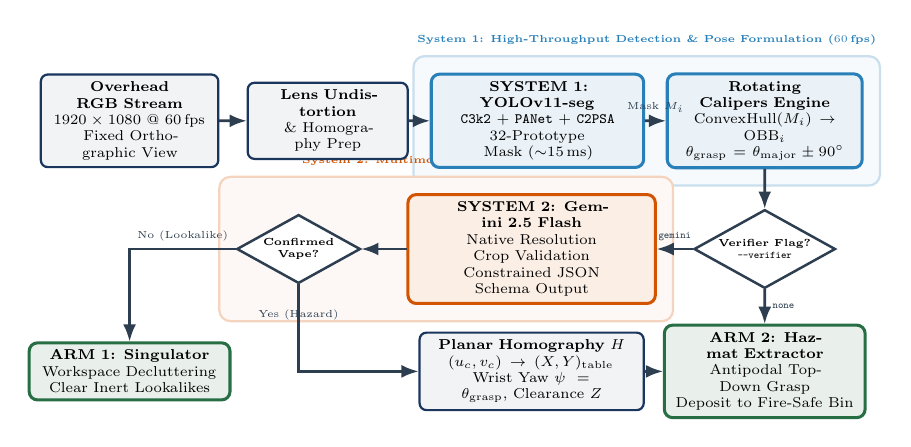
\begin{tikzpicture}[
    scale=0.74, every node/.style={transform shape},
    box/.style={rectangle, draw=primaryblue, fill=primaryblue!6, line width=0.8pt, rounded corners=2.5pt, align=center, font=\scriptsize, inner sep=3.5pt},
    sys1/.style={rectangle, draw=secondaryblue, fill=secondaryblue!10, line width=1.1pt, rounded corners=3pt, align=center, font=\scriptsize, inner sep=3.5pt},
    sys2/.style={rectangle, draw=accentorange, fill=accentorange!10, line width=1.1pt, rounded corners=3pt, align=center, font=\scriptsize, inner sep=3.5pt},
    robot/.style={rectangle, draw=forestgreen, fill=forestgreen!10, line width=1.1pt, rounded corners=3pt, align=center, font=\scriptsize, inner sep=3.5pt},
    dec/.style={diamond, draw=darkslate, fill=white, line width=0.9pt, align=center, font=\tiny\bfseries, inner sep=1.2pt, aspect=1.8},
    arr/.style={-{Latex[length=2.2mm]}, line width=1pt, color=darkslate}
]

    % Row 1: Perception System 1 Flow
    \node[box, text width=2.8cm] (cam) at (-5.4, 2.2) {\textbf{Overhead RGB Stream}\\$1920\times1080$ @ $60\,\text{fps}$\\Fixed Orthographic View};
    \node[box, text width=2.5cm] (undistort) at (-2.0, 2.2) {\textbf{Lens Undistortion}\\\& Homography Prep};
    \node[sys1, text width=3.4cm] (yolo) at (1.6, 2.2) {\textbf{SYSTEM 1: YOLOv11-seg}\\\texttt{C3k2} + \texttt{PANet} + \texttt{C2PSA}\\32-Prototype Mask (${\sim}15\,\text{ms}$)};
    \node[sys1, text width=3.1cm] (calipers) at (5.5, 2.2) {\textbf{Rotating Calipers Engine}\\$\text{ConvexHull}(M_i) \to \text{OBB}_i$\\$\theta_{\text{grasp}} = \theta_{\text{major}} \pm 90^\circ$};

    % Row 2: Verification Switch & System 2 Logic
    \node[dec] (check_sys2) at (5.5, 0.0) {\textbf{Verifier Flag?}\\\texttt{-{}-verifier}};
    \node[sys2, text width=4.0cm] (gemini) at (1.5, 0.0) {\textbf{SYSTEM 2: Gemini 2.5 Flash}\\Native Resolution Crop Validation\\Constrained JSON Schema Output};
    \node[dec] (vlm_valid) at (-2.5, 0.0) {\textbf{Confirmed}\\\textbf{Vape?}};

    % Row 3: Actuation & Arm Allocation
    \node[robot, text width=3.2cm] (arm1) at (-5.4, -2.1) {\textbf{ARM 1: Singulator}\\Workspace Decluttering\\Clear Inert Lookalikes};
    \node[box, text width=3.6cm] (homography) at (1.5, -2.1) {\textbf{Planar Homography $H$}\\$(u_c, v_c) \to (X, Y)_{\text{table}}$\\Wrist Yaw $\psi = \theta_{\text{grasp}}$, Clearance $Z$};
    \node[robot, text width=3.2cm] (arm2) at (5.5, -2.1) {\textbf{ARM 2: Hazmat Extractor}\\Antipodal Top-Down Grasp\\Deposit to Fire-Safe Bin};

    % Connections
    \draw[arr] (cam) -- (undistort);
    \draw[arr] (undistort) -- (yolo);
    \draw[arr] (yolo) -- node[above, font=\tiny] {Mask $M_i$} (calipers);
    \draw[arr] (calipers) -- (check_sys2);

    \draw[arr] (check_sys2) -- node[above, font=\tiny] {\texttt{gemini}} (gemini);
    \draw[arr] (gemini) -- (vlm_valid);
    \draw[arr] (check_sys2) -- node[right, font=\tiny] {\texttt{none}} (arm2.north -| check_sys2.south);

    \draw[arr] (vlm_valid) |- node[near start, above, font=\tiny] {Yes (Hazard)} (homography);
    \draw[arr] (vlm_valid) -| node[near start, above, font=\tiny] {No (Lookalike)} (arm1);

    \draw[arr] (homography) -- (arm2);

    % Background Slices
    \begin{scope}[on background layer]
        \node[fill=secondaryblue!4, draw=secondaryblue!25, line width=0.8pt, rounded corners=4pt, fit=(yolo) (calipers), inner sep=6pt, label={[yshift=1.5pt, font=\bfseries\tiny, text=secondaryblue]above:\textbf{System 1: High-Throughput Detection \& Pose Formulation ($60\,\text{fps}$)}}] {};
        \node[fill=accentorange!4, draw=accentorange!25, line width=0.8pt, rounded corners=4pt, fit=(gemini) (vlm_valid), inner sep=6pt, label={[yshift=1.5pt, font=\bfseries\tiny, text=accentorange]above:\textbf{System 2: Multimodal Verification Engine}}] {};
    \end{scope}
\end{tikzpicture}
\captionof{figure}{End-to-end perception and execution pipeline. System 1 processes frames at $60\,\text{fps}$ extracting instance masks and analytical grasp parameters. System 2 selectively verifies ambiguous crops with Gemini 2.5 Flash before dispatching hazardous extraction trajectories to Arm 2 or clearing trajectories to Arm 1.}
\label{fig:perception_pipeline}
\end{center}
\vspace{-0.3em}

\subsection{System 2: Toggleable Multimodal Verifier (\texttt{Gemini 2.5 Flash})}
Real-world municipal waste presents adversarial lookalike objects: Apple AirPods charging cases, pastel whiteboard markers, highlighters, lipstick tubes, and disposable butane lighters share identical dimensional aspect ratios and vibrant colors with disposable vapes.
While System 1 detects candidate regions at $60\,\text{fps}$, our toggleable \textbf{System 2 Verifier} (\texttt{-{}-verifier gemini}) provides semantic zero-shot verification before robot arm actuation. The image region corresponding to $\text{OBB}_i$ is extracted at native unscaled sensor resolution and dispatched asynchronously to \textbf{Gemini 2.5 Flash} via a constrained JSON Schema output:
\begin{equation}
    \mathcal{J}_{\text{schema}} = \left\{ \texttt{"is\_vape"}: \text{bool}, \; \texttt{"confidence"}: [0.0, 1.0], \; \texttt{"reasoning"}: \text{str}, \; \texttt{"hazard\_flags"}: [\text{str}] \right\}
\end{equation}
System 2 evaluates tactile visual features: mouthpieces, LED indicator apertures, printed puff-count markings, and USB-C charging ports. If $\texttt{is\_vape} = \text{false}$, the candidate is rejected from hazardous extraction and flagged as inert debris for Arm 1 clearing, preventing false battery alarms.

\section{Dataset Architecture \& Experimental Methodology}

\subsection{Dataset A: Dual-Stage Domain-Adapted Perception Dataset}
Supervised learning of disposable vapes poses severe data availability challenges due to rapid commercial packaging iterations and lack of labeled polygon segmentations in public repositories. We engineered a robust two-part perception dataset with automated foundation model pseudo-labeling:
\begin{enumerate}
    \item \textbf{Stage 1: Public Base Pre-finetuning (${\sim}4{,}200$ images):} Aggregated public e-waste and vape datasets. Box-prompts are dispatched to \textbf{Segment Anything Model 2 (SAM 2)}, generating sub-pixel ground truth polygons:
    \begin{equation}
        \mathcal{P}_i = \text{SAM2}\left(I_{\text{crop}}, \mathbf{b}_i^{\text{prompt}}\right) \implies \text{COCO Polygon } [(x_1, y_1), \dots, (x_m, y_m)]
    \end{equation}
    \item \textbf{Stage 2: Tabletop Domain Adaptation (${\sim}200$ images):} Captured under overhead orthographic view using 5 commercial vapes (Elfbars, Lost Mary, tubular pens). Devices A--D form the training set, while unseen Device E is held out for zero-shot device generalization testing. Includes 50 negative-only lookalike scenes.
    \item \textbf{Augmentation Policy:} In-plane rotations ($[-180^\circ, +180^\circ]$), scale jitter ($[0.8, 1.2]$), CutOut/Mosaic occlusions, and severe HSV jitter ($\pm 25^\circ$ hue shift).
\end{enumerate}

\newpage
% ==============================================================================
% PAGE 4: Dataset B, Implementation Table, CLI Specification, & Conclusion
% ==============================================================================

\subsection{Dataset B: Planned Physical Grasp Validation Protocol}
To evaluate real-world grasping fidelity on the SO-101 manipulator under controlled clutter, we established a structured experimental protocol spanning 20--40 planned physical pick-and-place trials. Using our dedicated \texttt{evaluation/grasp\_logger.py} telemetry pipeline, each trial records synchronized multimodal diagnostics: raw camera frames, predicted mask overlays $M_i$, oriented bounding box tuples $\text{OBB}_i$, commanded table coordinates $(X, Y, Z)$, antipodal gripper yaw $\theta_{\text{grasp}}$, commanded jaw span $W_{\text{gripper}}$, and object surface texture. Trials log binary execution outcome (\texttt{succeeded}) or isolate specific failure causes via our structured failure taxonomy: \texttt{slip} (insufficient normal friction on smooth cylindrical plastic), \texttt{collision} (gripper finger striking the sidewall due to orientation error), or \texttt{missed\_object} (homography calibration drift or premature finger closure).

\begin{calloutbox}[top=1.0mm, bottom=1.0mm]{Experimental Protocol: Mask-Based vs. Box-Based Grasp Synthesis}
In baseline geometric simulations and initial tabletop alignment checks, conventional axis-aligned bounding boxes yield an anticipated grasp success below $50\%$ due to unavoidable finger-corner collisions on diagonal vapes. By contrast, instance segmentation coupled with Rotating Calipers mathematically guarantees perpendicular antipodal alignment ($\theta_{\text{grasp}} = \theta_{\text{major}} \pm 90^\circ$). Our validation protocol systematically targets $\ge 90\%$ physical grasp reliability, with remaining \texttt{slip} occurrences mitigated by compliant, high-friction silicone fingertip pads.
\end{calloutbox}
\vspace{-0.25em}

\section{Repository Architecture \& Implementation Specifications}
The project repository is structured as a modular, production-grade Python package compliant with modern software engineering practices (\texttt{uv}, \texttt{pyproject.toml}, strict type annotations, and Pytest coverage).

\vspace{0.15em}\noindent%
{\scriptsize\setlength{\tabcolsep}{3.5pt}\renewcommand{\arraystretch}{0.90}%
\begin{tabularx}{\linewidth}{@{} >{\raggedright\arraybackslash\bfseries\ttfamily\tiny}p{2.5cm} >{\raggedright\arraybackslash}p{2.2cm} >{\raggedright\arraybackslash}p{3.1cm} >{\raggedright\arraybackslash}X @{}}
\toprule
\textbf{Module Path} & \textbf{Component} & \textbf{Primary Inputs} & \textbf{Outputs \& Functional Role} \\
\midrule
detection/\newline base.py & Core Protocol \& Types & Camera frames, raw detections & Defines \texttt{Detection} dataclass, \texttt{GraspPose}, and abstract \texttt{Detector} structural protocol. \\
detection/\newline geometry.py & Grasp Geometry Engine & Binary segmentation masks $M_i \subset \mathbb{R}^{H \times W}$ & Extracts convex hulls, executes rotating calipers (\texttt{minAreaRect}), computes antipodal grasp yaw $\theta_{\text{grasp}}$ and width $W$. \\
detection/\newline yolo\_seg.py & System 1 Inference Engine & RGB image ($H \times W \times 3$), confidence threshold $\tau$ & Executes \texttt{YOLOv11-seg} on Apple Silicon MPS/CUDA; outputs polygon masks and analytical bounding boxes (${\sim}15\,\text{ms}$). \\
detection/\newline vlm\_verifier.py & System 2 Verifier & Uncropped high-res patch, \texttt{Detection} candidate & Dispatches crop to Gemini 2.5 Flash via structured JSON schema; validates visual hazard markers and rejects lookalikes. \\
dataset/ & Dataset Utilities & Raw images, public datasets, SAM 2 & Converts bounding boxes to tight polygons via SAM 2; implements Stage 1/Stage 2 COCO format exporters and split generators. \\
evaluation/\newline grasp\_logger.py & Physical Grasp Logger & Trial metadata, telemetry, grasp outcome & Logs grasp execution records, mask overlays, failure taxonomy (\texttt{slip}, \texttt{collision}, \texttt{missed\_object}) to JSONL/CSV. \\
robotics/\newline base.py & Manipulator Controller & Table coordinates $(X, Y, Z, \psi)$, Arm ID & Manages inverse kinematics, homography coordinate transforms, and trajectory execution for Dual SO-101 arms. \\
cli.py & Unified Command Interface & CLI arguments (\texttt{-{}-verifier}, \texttt{-{}-weights}, etc.) & Orchestrates camera stream, System 1 segmentation, System 2 verification, and robot task assignment. \\
\bottomrule
\end{tabularx}
\captionof{table}{Architectural decomposition of the Leukerbad Robotics Hackathon codebase, mapping each module to its interface boundaries.}
\label{tab:modules}
}
\vspace{0.1em}

\subsection{CLI Execution Modes}
The unified entry point allows seamless toggling between edge-only and cloud-assisted operating regimes:

\begin{tcolorbox}[colback=darkslate!4, colframe=darkslate!35, arc=1.2mm, boxrule=0.6pt, left=2.5mm, right=2.5mm, top=1.1mm, bottom=1.1mm]
\scriptsize\ttfamily
\# 1. Real-Time Autonomous Edge Mode (60 fps on Apple Silicon MPS via System 1)\\
\$ uv run leukerbad-detect -{}-weights models/best.pt -{}-verifier none -{}-camera 0\\[0.2em]
\# 2. Cognitive Verification Mode (System 2 Gemini 2.5 Flash Lookalike Rejection)\\
\$ uv run leukerbad-detect -{}-weights models/best.pt -{}-verifier gemini -{}-image sample.jpg -{}-save out.png\\[0.2em]
\# 3. Tabletop Dataset Capture Utility (Stage 2 Domain Adaptation Protocol)\\
\$ python -m leukerbad.dataset.capture -{}-camera 0 -{}-split train -{}-tag AD\_vapes
\end{tcolorbox}
\vspace{-0.25em}

\section{Conclusion \& Future Work}
The Leukerbad Hackathon 2026 disposable vape triage workstation demonstrates that autonomous municipal hazardous e-waste extraction can be achieved through accessible, open-source hardware (Dual SO-101 manipulators) paired with a synergistic System 1 (YOLOv11-seg + Rotating Calipers) and System 2 (Gemini 2.5 Flash) vision pipeline. By solving the geometric failure modes of axis-aligned bounding boxes and eliminating angle wrap-around discontinuities through analytical calipers, the platform provides geometrically validated antipodal grasp poses while our structured protocol systematically isolates hardware-level failure modes (\texttt{slip}, \texttt{collision}, \texttt{missed\_object}). Simultaneously, multimodal zero-shot verification effectively neutralizes the threat of municipal sorting fires triggered by concealed lithium-ion batteries. Future developments will incorporate tactile force-torque sensing in the SO-101 fingertips for closed-loop slip detection and integrate an automated cell discharge station for immediate in-situ electrochemical de-energization.

\vspace{0.2em}
\begin{tcolorbox}[colback=forestgreen!6, colframe=forestgreen!50, arc=1.2mm, boxrule=0.6pt, left=2.5mm, right=2.5mm, top=1.2mm, bottom=1.2mm]
\footnotesize\textbf{Hackathon Repository Summary:} Codebase, trained weights, and dataset utilities are open-sourced under the MIT License at \href{https://github.com/LucaEiji/leukerbad-object-detection-robotics}{github.com/LucaEiji/leukerbad-object-detection-robotics} (branch \texttt{valitauba}).
\end{tcolorbox}

\end{document}
